\section{Descrizione del progetto}
Per quanto riguarda il progetto realizzato in cpp si è pensato, piuttosto che realizzare un applicativo "funzionale" (approccio seguito per gli altri 3 progetti), di andare a realizzare, come oggetto di questo elaborato, una libreria per il calcolo numerico, che consiste in due moduli principali:
\begin{itemize}
	\item Matrici
	\item Applicativo dimostrativo
\end{itemize}

In particolare sono state sviluppate alcune funzionalità algebriche base come \textit{sommma} e \textit{sottrazione} elemento per elemento di una matrice: l'espressività del C++ ha permesso di rendere questa libreria del tutto generica, permettendo quindi di realizzare matrici composte da elementi di qualsiasi tipo, tramite l'utilizzo dei \textit{templetes generici}.

\section{Gerarchia delle classi}
Come si vede nell'\textit{UML Class Diagram} in figura ~\ref{fig:UMLClassDiagram}, la libreria presenta una classe base principale, \textit{Number}, che rappresenta un numero il quale può essere un numero di tipo \textit{Addable} o \textit{Subtractable}, che offrono rispettivamente un metodo e un operatore per realizzare la somma e la sottrazione.
\begin{figure}[h]
	\centering
	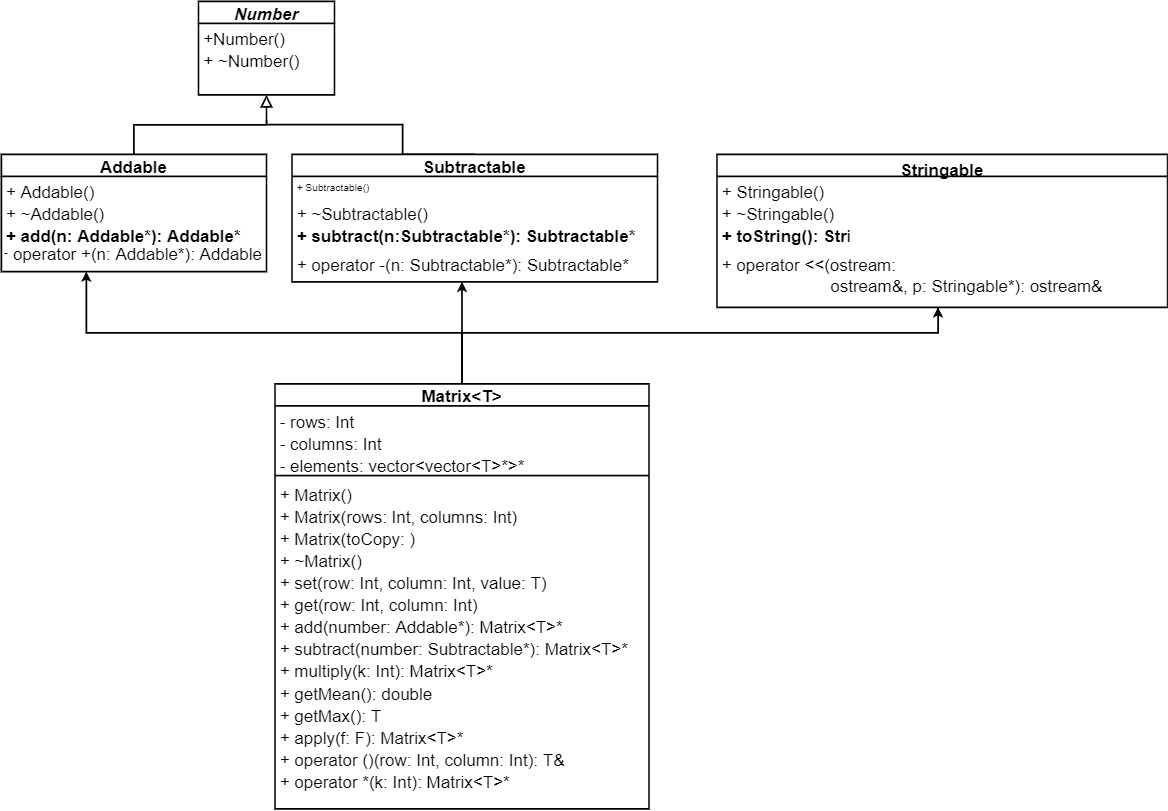
\includegraphics[width=0.7\textwidth]{Immagini/ClassDiagram.jpg}
	\caption{UML class diagram}
	\label{fig:UMLClassDiagram}
\end{figure}

\section{Multiple inheritance}
Nella gerarchia delle classi esposta sopra, è stato necessario utilizzare l’ereditarietà multipla
nei due diversi contesti tipici: 
\begin{itemize}
	\item implementazione di interfacce
	\item ereditarietà multipla \textit{classica}
\end{itemize}

Il C++ non fa distinzioni sostanziali tra queste due tipologie, ma la differenza concettuale è
notevole, tanto che altri linguaggi (come Java) permettono il primo tipo di ereditarietà multipla
e non il secondo.

La prima tipologia consiste nel derivare una classe da al più una classe base “non pure virtual”.
Le altre classi base devono essere l’equivalente delle interface Java, ovvero devono essere
classi astratte (\textit{Abstract Base Classes} - ABCs) in cui tutte le member functions (o quasi) sono
pure virtual e in cui tutte le member variables sono costanti e pubbliche.

Questa tipologia di eredità è stata utilizzata per derivare da Stringable.

La seconda tipologia di eredità è stata invece utilizzata per andare a modellizzare il rapporto tra una matrice e quelle che sono le strutture relative a \textit{Number}, come si vede nella figura ~\ref{fig:MultipleInerithance}.

\begin{figure}[h]
	\centering
	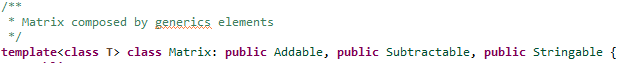
\includegraphics[width=0.6\textwidth]{Immagini/MultipleInerithance.png}
	\caption{Esempio di eredità multipla della classe \textit{Matrix}}
	\label{fig:MultipleInerithance}
\end{figure}

\section{Diamond inheritance}
Un aspetto problematico dell’ereditarietà multipla (specialmente per il secondo tipo) è la
possibilità di generare una gerarchia a diamante.

Esso si verifica quando, come si vede nella figura ~\ref{fig:DiamondProblem} una generica classe D eredita da due classi B e C che hanno un antenato in
comune A. In questo caso c'è un'ambiguità su quale “versione” dell'antenato deve essere ereditata
da D: quella di B o quella di C?

\begin{figure}[h]
	\centering
	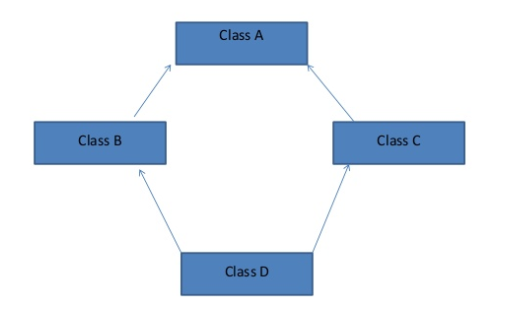
\includegraphics[width=0.3\textwidth]{Immagini/DiamondProblem.png}
	\caption{Diamond problem}
	\label{fig:DiamondProblem}
\end{figure}

Un modo di risolvere il problema in C++ è dichiarare, nelle classi B e C, un'eredità \textit{virtuale} da A, specificandolo direttamente nella dichiarazione, come fatto nelle classi \textit{Addble} e \textit{Subtractable} (figura ~\ref{fig:VirtualInerithance}).

\begin{figure}[h]
	\centering
	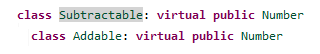
\includegraphics[width=0.5\textwidth]{Immagini/VirtualInerithance.png}
	\caption{Virtual Inerithance nelle classe \textit{Addable} e \textit{Subtractable}}
	\label{fig:VirtualInerithance}
\end{figure}


L’ereditarietà virtuale introduce comunque un altro leggero problema: poiché esiste un’unica
classe base, le classi derivate direttamente da essa non possono inizializzare l’oggetto della
classe base, perché si avrebbe un conflitto tra queste inizializzazioni. Il compito di costruire
l’istanza della classe base è quindi delegato alla classe most-derived, ovvero a quella che sta
alla “convergenza” dei rami del diamante. Ciò che è più contro intuitivo è che anche eventuali
classi derivate da quest’ultima (anche con ereditarietà singola) devono inizializzare
direttamente la virtual base class; questo può rendere poco chiaro il codice e richiedere alle
classi derivate di conoscere alcuni dettagli della virtual base class che altrimenti potrebbero
ignorare.

\section{Virtual method}
In C++, una sottoclasse può sempre ridefinire i metodi della sopraclasse, ma il dynamic binding non
avviene se non si usa la parola chiave virtual (a differenza di Java dove avviene sempre).

Pertanto, ogni metodo che viene (o potrebbe essere) ridefinito in una sottoclasse va dichiarato come virtuale.
Un caso particolare è il distruttore, che se non fosse virtuale non permetterebbe la distruzione di
tutti gli oggetti appartenenti alle sottoclassi: per questo che, nella classe base \textit{Number} il distruttore è stato dichiarato di tipo virtual come si vede in figura ~\ref{fig:VirtualDesctructor}

\begin{figure}[h]
	\centering
	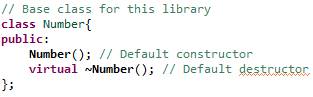
\includegraphics[width=0.5\textwidth]{Immagini/VirtualDestructor.png}
	\caption{Virtual desctructor della classe base \textit{Number}}
	\label{fig:VirtualDesctructor}
\end{figure}

L'utilizzo di metodo virtuale ne permette anche l'applicazione e l'utilizzo come interfacce Java, tramite i metodi \textit{virtual pure}: in particolare, questi metodi virtuali, possono essere usati proprio come gli altri, con la differenza che le classi contenenti metodi virtuali puri non possono però essere istanziate.

\section{Overloading particolari}
Nella nostra libreria, su consigli di altri studenti, siamo andati a ridefinire alcuni operatori, per renderli più "personalizzati".
\subsection{Overloading di cout<<}
Tra gli operatori che risulta utili sovraccaricare c'è \textit{"<<"}, il quale è utilizzato nella libreria standard per inviare dati agli oggetti \textit{ostream} (flussi in output): è stato quindi possibile personalizzare, in maniera facile e diffusa, la tipologia di log aggiungendo, coem si vede in figura ~\ref{fig:CoutRedef}, 

\begin{figure}[h]
	\centering
	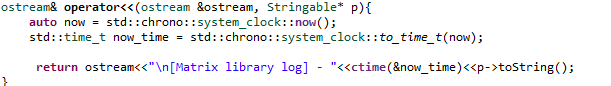
\includegraphics[width=0.5\textwidth]{Immagini/CoutRedefinition.png}
	\caption{Ridefinizione dell'operatore di stream}
	\label{fig:CoutRedef}
\end{figure}

\subsection{Overloading di ()}
L'operatore () è leggeremente diverso dagli altri, in quanto è possibile interpretarli in due modi, a seconda che compaiano in un l-value o in un r-value.

In C++ è possibile sovraccaricare gli operatori in modo che si comportino in maniera diversa a seconda della posizione esattamente come accade con gli array.

\begin{figure}[h]
	\centering
	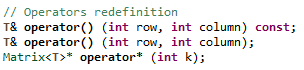
\includegraphics[width=0.3\textwidth]{Immagini/MatrixOperatorsRedef.png}
	\caption{Ridefinizione degli operatori nella classe \textit{Matrix}}
	\label{fig:MatrixOperatorRedef}
\end{figure}

Nella nostra applicazione siamo andati a ridefinire appunto l'operatore (), come si vede in figura ~\ref{fig:MatrixOperatorRedef}, in particolare:
\begin{itemize}
	\item  la presenza del simbolo $\&$ subito dopo il valore ritornato indica che ci sono due definizioni diverse dello stesso operatore.
	\item il modificatore const indica invece che la prima ridefinizione è quella da usare se l'operatore sta a sinistra del simbolo di assegnamento.
\end{itemize}
Esempi di utilizzo della redefinizione dell'operatore (), li si possono vedere in figura ~\ref{fig:OperatorExamples}.

\begin{figure}[h]
	\centering
	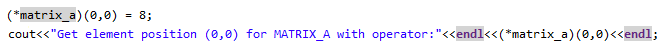
\includegraphics[width=0.5\textwidth]{Immagini/OperatorExample.png}
	\caption{Esempio di utilizzo della redefinizione degli operatori}
	\label{fig:OperatorExamples}
\end{figure}

\section{Templates}
Un metodo più potente per il riutilizzo del codice è fornito dai templates. Essi costituiscono
uno “schema” di classe che poi verrà realizzato concretamente sostituendo ai tipi parametrici i
tipi effettivi dichiarati dagli utilizzatori del template

A differenza del linguaggio Java, ogni differente realizzazione del template costituisce un tipo
a sé stante e senza alcuna relazione con gli altri. In Java si può avere una gerarchia di tipi
derivati dallo stesso template.

In C++ invece ogni realizzazione di un template viene concretizzata tramite codice
indipendente, portando quindi ad un file eseguibile di dimensioni maggiori. Inoltre, per fornire
vincoli in modo esplicito come in Java, si deve ricorrere a una “pseudo-ereditarietà”.

Questa flessibilità offerta dai templates, è stata utilizzata nella stesura della classe \textit{Matrix}.

\section{Standard Template Library}
La libreria STL del C++ mette a disposizione una serie di contenitori parametrici, che quindi
possono contenere oggetti di tipo arbitrario. Fornisce inoltre iteratori che permettono di visitare
tali contenitori e algoritmi per manipolarne gli elementi.

Uno dei contenitori più semplici è \textit{vector}, una classe che permette di gestire collezioni di oggetti ordinati come un array.

I vantaggi del vector sul semplice array sono diversi, tra cui la gestione automatica della
memoria e la presenza di diversi metodi per le operazioni più comuni quali l'inserimento di un
nuovo valore.

La classe Matrix utilizza un vector per memorizzare gli elementi della matrice ed essendo
parametrica di parametro T, utilizza un \textit{vector<vector<T>>}.
\subsection{STL - Iterator}
Tra le altre funzionalità messe a disposizione da vector e dagli altri contenitori in STL ci sono gli
iteratori, che costituiscono il modo standard di accedere agli elementi nel contenitore stesso. Gli
iteratori si comportano in modo simile a semplici puntatori (ad esempio ammettono l'operatore ++),
anche se in realtà sono più flessibili e possono essere utilizzati anche con le liste.

\begin{figure}[h]
	\centering
	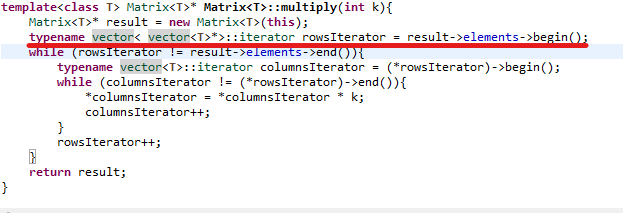
\includegraphics[width=0.7\textwidth]{Immagini/Stl_Iterator.png}
	\caption{STL - Iterator}
	\label{fig:Iterator}
\end{figure}

\subsection{STL - Algorithm}
La libreria STL mette a disposizione anche degli algoritmi generici e riutilizzabili per operare sui contenitori.

Tali algoritmi sono implementati tramite funzioni template che si possono includere nei propri file tramite la direttiva di include.

Un esempio di algoritmo è la funzione \textit{for-each()}, che applica una funzione parametro a tutti gli
elementi di un contenitore.

\begin{figure}[h]
	\centering
	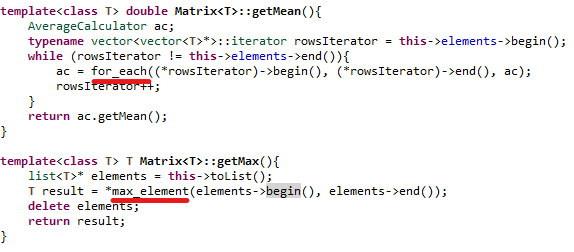
\includegraphics[width=0.7\textwidth]{Immagini/Stl_Algorithm.png}
	\caption{STL - Algorithm}
	\label{fig:Algoritm}
\end{figure}